\documentclass{standalone}
\usepackage{tikz}
\usetikzlibrary{patterns, positioning}


\begin{document}
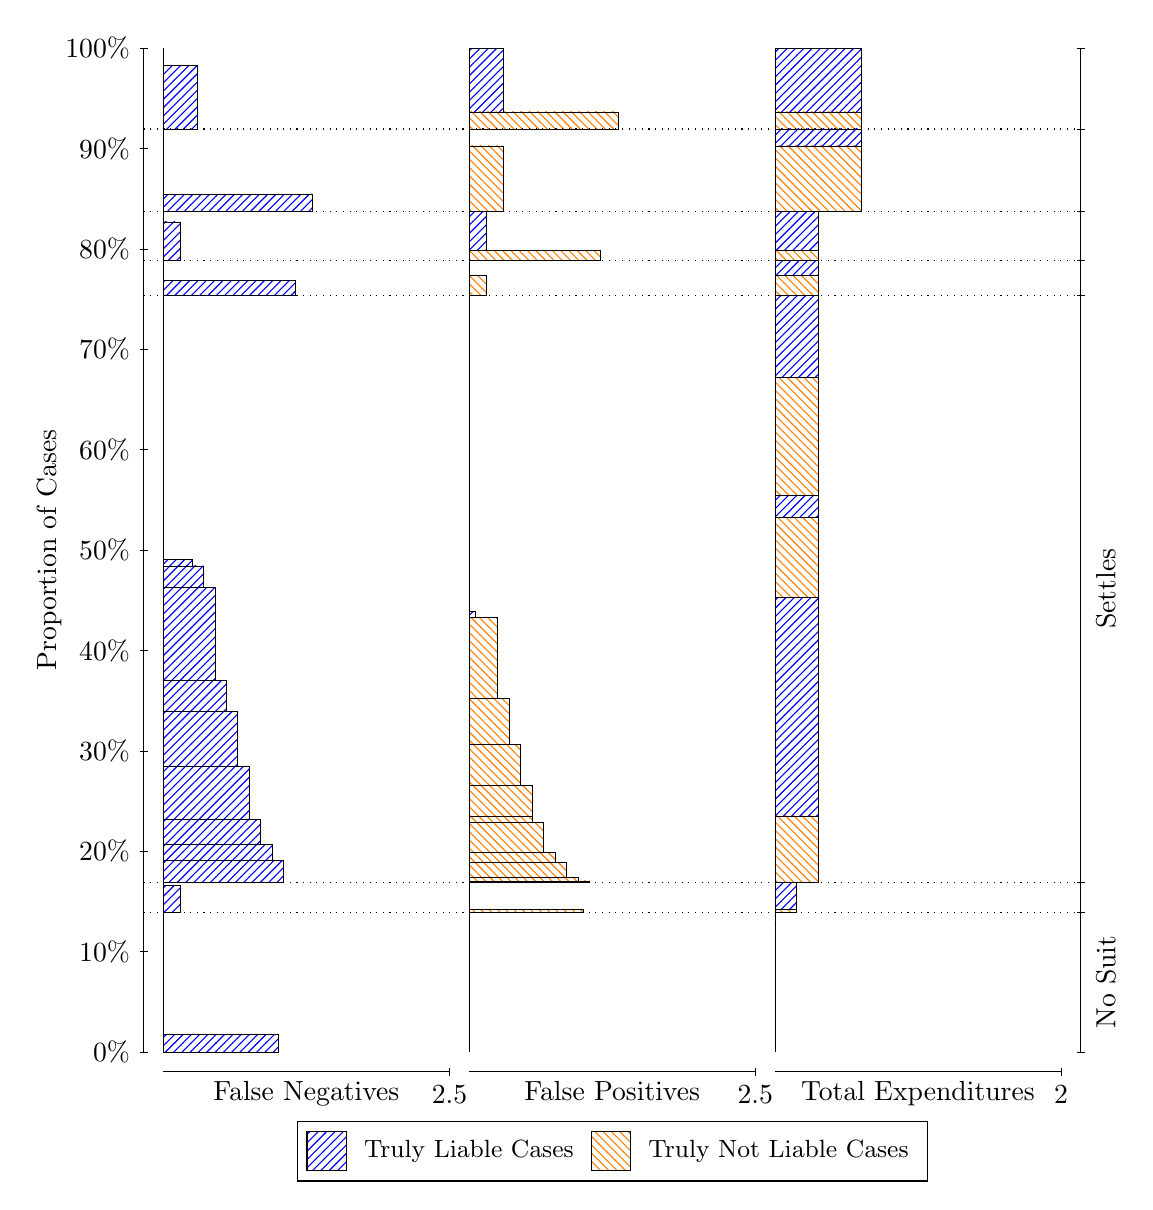
\begin{tikzpicture}
\draw[black, very thin] (1.5,1.75) -- (1.5,14.5);
\node[rotate=90, text=black, anchor=center] at (0.3, 8.125) {Proportion of Cases};
\draw[black, very thin] (1.45,1.75) -- (1.55,1.75);
\node[text=black, anchor=east] at (1.45, 1.75) {0\%};
\draw[black, very thin] (1.45,3.025) -- (1.55,3.025);
\node[text=black, anchor=east] at (1.45, 3.025) {10\%};
\draw[black, very thin] (1.45,4.3) -- (1.55,4.3);
\node[text=black, anchor=east] at (1.45, 4.3) {20\%};
\draw[black, very thin] (1.45,5.575) -- (1.55,5.575);
\node[text=black, anchor=east] at (1.45, 5.575) {30\%};
\draw[black, very thin] (1.45,6.85) -- (1.55,6.85);
\node[text=black, anchor=east] at (1.45, 6.85) {40\%};
\draw[black, very thin] (1.45,8.125) -- (1.55,8.125);
\node[text=black, anchor=east] at (1.45, 8.125) {50\%};
\draw[black, very thin] (1.45,9.4) -- (1.55,9.4);
\node[text=black, anchor=east] at (1.45, 9.4) {60\%};
\draw[black, very thin] (1.45,10.675) -- (1.55,10.675);
\node[text=black, anchor=east] at (1.45, 10.675) {70\%};
\draw[black, very thin] (1.45,11.95) -- (1.55,11.95);
\node[text=black, anchor=east] at (1.45, 11.95) {80\%};
\draw[black, very thin] (1.45,13.225) -- (1.55,13.225);
\node[text=black, anchor=east] at (1.45, 13.225) {90\%};
\draw[black, very thin] (1.45,14.5) -- (1.55,14.5);
\node[text=black, anchor=east] at (1.45, 14.5) {100\%};

\draw[black, very thin] (13.4,1.75) -- (13.4,14.5);
\draw[black, very thin] (13.35,1.75) -- (13.45,1.75);
\node[anchor=west] at (13.35, 1.75) {};
\draw[black, very thin] (13.35,3.5246) -- (13.45,3.5246);
\node[anchor=west] at (13.35, 3.5246) {};
\draw[black, very thin] (13.35,3.9058) -- (13.45,3.9058);
\node[anchor=west] at (13.35, 3.9058) {};
\draw[black, very thin] (13.35,11.362) -- (13.45,11.362);
\node[anchor=west] at (13.35, 11.362) {};
\draw[black, very thin] (13.35,11.799) -- (13.45,11.799);
\node[anchor=west] at (13.35, 11.799) {};
\draw[black, very thin] (13.35,12.421) -- (13.45,12.421);
\node[anchor=west] at (13.35, 12.421) {};
\draw[black, very thin] (13.35,13.472) -- (13.45,13.472);
\node[anchor=west] at (13.35, 13.472) {};
\draw[black, very thin] (13.35,14.5) -- (13.45,14.5);
\node[anchor=west] at (13.35, 14.5) {};

\draw[black, very thin, pattern color=blue, pattern=north east lines] (1.75,1.75) rectangle (3.2033,1.9773);
\draw[black, very thin, pattern color=orange, pattern=north west lines] (1.75,1.9773) rectangle (1.75,3.5246);
\draw[black, very thin, pattern color=blue, pattern=north east lines] (1.75,3.5246) rectangle (1.968,3.8667);
\draw[black, very thin, pattern color=orange, pattern=north west lines] (1.75,3.8667) rectangle (1.75,3.9058);
\draw[black, very thin, pattern color=blue, pattern=north east lines] (1.75,3.9058) rectangle (3.276,4.1858);
\draw[black, very thin, pattern color=blue, pattern=north east lines] (1.75,4.1858) rectangle (3.1307,4.3847);
\draw[black, very thin, pattern color=blue, pattern=north east lines] (1.75,4.3847) rectangle (2.9853,4.7007);
\draw[black, very thin, pattern color=blue, pattern=north east lines] (1.75,4.7007) rectangle (2.84,5.3769);
\draw[black, very thin, pattern color=blue, pattern=north east lines] (1.75,5.3769) rectangle (2.6947,6.0708);
\draw[black, very thin, pattern color=blue, pattern=north east lines] (1.75,6.0708) rectangle (2.5493,6.4731);
\draw[black, very thin, pattern color=blue, pattern=north east lines] (1.75,6.4731) rectangle (2.404,7.647);
\draw[black, very thin, pattern color=blue, pattern=north east lines] (1.75,7.647) rectangle (2.2587,7.9219);
\draw[black, very thin, pattern color=blue, pattern=north east lines] (1.75,7.9219) rectangle (2.1133,8.0031);
\draw[black, very thin, pattern color=orange, pattern=north west lines] (1.75,8.0031) rectangle (1.75,11.362);
\draw[black, very thin, pattern color=blue, pattern=north east lines] (1.75,11.362) rectangle (3.4213,11.55);
\draw[black, very thin, pattern color=orange, pattern=north west lines] (1.75,11.55) rectangle (1.75,11.799);
\draw[black, very thin, pattern color=blue, pattern=north east lines] (1.75,11.799) rectangle (1.968,12.291);
\draw[black, very thin, pattern color=orange, pattern=north west lines] (1.75,12.291) rectangle (1.75,12.421);
\draw[black, very thin, pattern color=blue, pattern=north east lines] (1.75,12.421) rectangle (3.6393,12.637);
\draw[black, very thin, pattern color=orange, pattern=north west lines] (1.75,12.637) rectangle (1.75,13.472);
\draw[black, very thin, pattern color=blue, pattern=north east lines] (1.75,13.472) rectangle (2.186,14.284);
\draw[black, very thin, pattern color=orange, pattern=north west lines] (1.75,14.284) rectangle (1.75,14.5);
\draw[black, very thin, pattern color=orange, pattern=north west lines] (5.6333,1.75) rectangle (5.6333,3.2973);
\draw[black, very thin, pattern color=blue, pattern=north east lines] (5.6333,3.2973) rectangle (5.6333,3.5246);
\draw[black, very thin, pattern color=orange, pattern=north west lines] (5.6333,3.5246) rectangle (7.0867,3.5637);
\draw[black, very thin, pattern color=blue, pattern=north east lines] (5.6333,3.5637) rectangle (5.6333,3.9058);
\draw[black, very thin, pattern color=orange, pattern=north west lines] (5.6333,3.9058) rectangle (7.1593,3.9227);
\draw[black, very thin, pattern color=orange, pattern=north west lines] (5.6333,3.9227) rectangle (7.014,3.9687);
\draw[black, very thin, pattern color=orange, pattern=north west lines] (5.6333,3.9687) rectangle (6.8687,4.1598);
\draw[black, very thin, pattern color=orange, pattern=north west lines] (5.6333,4.1598) rectangle (6.7233,4.2838);
\draw[black, very thin, pattern color=orange, pattern=north west lines] (5.6333,4.2838) rectangle (6.578,4.6678);
\draw[black, very thin, pattern color=orange, pattern=north west lines] (5.6333,4.6678) rectangle (6.4327,4.7469);
\draw[black, very thin, pattern color=orange, pattern=north west lines] (5.6333,4.7469) rectangle (6.4327,5.1317);
\draw[black, very thin, pattern color=orange, pattern=north west lines] (5.6333,5.1317) rectangle (6.2873,5.6545);
\draw[black, very thin, pattern color=orange, pattern=north west lines] (5.6333,5.6545) rectangle (6.142,6.2432);
\draw[black, very thin, pattern color=orange, pattern=north west lines] (5.6333,6.2432) rectangle (5.9967,7.2645);
\draw[black, very thin, pattern color=blue, pattern=north east lines] (5.6333,7.2645) rectangle (5.706,7.3458);
\draw[black, very thin, pattern color=blue, pattern=north east lines] (5.6333,7.3458) rectangle (5.6333,11.362);
\draw[black, very thin, pattern color=orange, pattern=north west lines] (5.6333,11.362) rectangle (5.8513,11.611);
\draw[black, very thin, pattern color=blue, pattern=north east lines] (5.6333,11.611) rectangle (5.6333,11.799);
\draw[black, very thin, pattern color=orange, pattern=north west lines] (5.6333,11.799) rectangle (7.3047,11.929);
\draw[black, very thin, pattern color=blue, pattern=north east lines] (5.6333,11.929) rectangle (5.8513,12.421);
\draw[black, very thin, pattern color=orange, pattern=north west lines] (5.6333,12.421) rectangle (6.0693,13.256);
\draw[black, very thin, pattern color=blue, pattern=north east lines] (5.6333,13.256) rectangle (5.6333,13.472);
\draw[black, very thin, pattern color=orange, pattern=north west lines] (5.6333,13.472) rectangle (7.5227,13.688);
\draw[black, very thin, pattern color=blue, pattern=north east lines] (5.6333,13.688) rectangle (6.0693,14.5);
\draw[black, very thin, pattern color=orange, pattern=north west lines] (9.5167,1.75) rectangle (9.5167,3.2973);
\draw[black, very thin, pattern color=blue, pattern=north east lines] (9.5167,3.2973) rectangle (9.5167,3.5246);
\draw[black, very thin, pattern color=orange, pattern=north west lines] (9.5167,3.5246) rectangle (9.7892,3.5637);
\draw[black, very thin, pattern color=blue, pattern=north east lines] (9.5167,3.5637) rectangle (9.7892,3.9058);
\draw[black, very thin, pattern color=orange, pattern=north west lines] (9.5167,3.9058) rectangle (10.062,4.7469);
\draw[black, very thin, pattern color=blue, pattern=north east lines] (9.5167,4.7469) rectangle (10.062,7.5219);
\draw[black, very thin, pattern color=orange, pattern=north west lines] (9.5167,7.5219) rectangle (10.062,8.5432);
\draw[black, very thin, pattern color=blue, pattern=north east lines] (9.5167,8.5432) rectangle (10.062,8.8233);
\draw[black, very thin, pattern color=orange, pattern=north west lines] (9.5167,8.8233) rectangle (10.062,10.32);
\draw[black, very thin, pattern color=blue, pattern=north east lines] (9.5167,10.32) rectangle (10.062,11.362);
\draw[black, very thin, pattern color=orange, pattern=north west lines] (9.5167,11.362) rectangle (10.062,11.611);
\draw[black, very thin, pattern color=blue, pattern=north east lines] (9.5167,11.611) rectangle (10.062,11.799);
\draw[black, very thin, pattern color=orange, pattern=north west lines] (9.5167,11.799) rectangle (10.062,11.929);
\draw[black, very thin, pattern color=blue, pattern=north east lines] (9.5167,11.929) rectangle (10.062,12.421);
\draw[black, very thin, pattern color=orange, pattern=north west lines] (9.5167,12.421) rectangle (10.607,13.256);
\draw[black, very thin, pattern color=blue, pattern=north east lines] (9.5167,13.256) rectangle (10.607,13.472);
\draw[black, very thin, pattern color=orange, pattern=north west lines] (9.5167,13.472) rectangle (10.607,13.688);
\draw[black, very thin, pattern color=blue, pattern=north east lines] (9.5167,13.688) rectangle (10.607,14.5);
\draw[black, dotted] (1.5,3.5246) -- (13.4,3.5246);
\draw[black, dotted] (1.5,3.9058) -- (13.4,3.9058);
\draw[black, dotted] (1.5,11.362) -- (13.4,11.362);
\draw[black, dotted] (1.5,11.799) -- (13.4,11.799);
\draw[black, dotted] (1.5,12.421) -- (13.4,12.421);
\draw[black, dotted] (1.5,13.472) -- (13.4,13.472);
\draw[black, very thin] (1.75,1.5) -- (5.3833,1.5);
\node[text=black, anchor=north] at (3.5667, 1.5) {False Negatives};
\draw[black, very thin] (5.3833,1.45) -- (5.3833,1.55);
\node[text=black, anchor=north] at (5.3833, 1.45) {2.5};

\draw[black, very thin] (5.6333,1.5) -- (9.2667,1.5);
\node[text=black, anchor=north] at (7.45, 1.5) {False Positives};
\draw[black, very thin] (9.2667,1.45) -- (9.2667,1.55);
\node[text=black, anchor=north] at (9.2667, 1.45) {2.5};

\draw[black, very thin] (9.5167,1.5) -- (13.15,1.5);
\node[text=black, anchor=north] at (11.333, 1.5) {Total Expenditures};
\draw[black, very thin] (13.15,1.45) -- (13.15,1.55);
\node[text=black, anchor=north] at (13.15, 1.45) {2};

\node[text=black, centered, rotate=90] at (13.72, 2.6373) {No Suit};

\node[text=black, centered, rotate=90] at (13.72, 7.6338) {Settles};





\draw (7.449999999999999,1.5) node[draw=none] (baseCoordinate) {};
\begin{scope}[align=center]
        \matrix[scale=0.5, draw=black, below=0.5cm of baseCoordinate, nodes={draw}, column sep=0.1cm]{
            \node[rectangle, draw, minimum width=0.5cm, minimum height=0.5cm, pattern color=blue, pattern=north east lines] {}; &
            \node[draw=none, font=\small, text=black] (B) {Truly Liable Cases}; &
            \node[rectangle, draw, minimum width=0.5cm, minimum height=0.5cm, pattern color=orange, pattern=north west lines] {}; &
            \node[draw=none, font=\small, text=black] (B) {Truly Not Liable Cases}; \\
            };
\end{scope}

\end{tikzpicture}
\end{document}